\section{Tipos de Autenticação}

\hspace{1cm} Nesta secção serão exploradas as diferentes categorias de fatores de autenticação, nomeadamente, algo que se sabe (PINs, passwords, etc.), algo que se é (Biometria) e algo que se possui (token fisico, cartão, etc.). 

\hspace{1cm} O exemplo mais comum de autenticação é a autenticação através de password, onde o utlizador autentica-se através da criação de um nome de utilizador e de uma password, e acede ao site/aplicação pretendida. Outro tipo de autenticação é a autenticação PIN, onde o utilizador, através de uma combinação de valores numéricos autentica-se e acede ao conteúdo pretendido.
A segurança destes exemplos depende dos requisistos requeridos pelo sistema de criação de utilizadores presente na aplicação. Boas práticas da criação de passwords/PINs, segundo o site "TechTarget - \textit{Single-factor authentication}" incluem a criação de um(a) PIN/password complexo/a e robusto/a de forma a que ninguém, através de ataques de força bruta, consiga descobri-la.

\hspace{1cm} Outro exemplo de um tipo de autenticação são os dados biometricos. Isto corresponde a características físicas, biológicas ou comportamentais únicas de um indivíduo que podem ser medidas e usadas para identificação, pois são considerados são únicos e exclusivos a cada indivíduo. Com isto, a autenticação através de dados biométricos corresponde a uma ferramenta valiosa para autenticação e segurança, apesar de não serem completamente invulneráveis a ameaças.

\hspace{1cm} Por fim, um outro tipo de autenticação corresponde à utilização de um token físico, ou token de hardware, que corresponde a um componente de hardware que autentica um utilizador. 
Os tokens físicos podem assumir várias formas, incluindo pequenos tokens USB, cartões inteligentes ou dispositivos dedicados que geram senhas. Os tokens físicos geralmente funcionam junto com outros métodos de autenticação, como um nome de usuário e uma senha, mas alguns sistemas podem usá-los como o único método de autenticação necessário.

\section{Autenticação Simples e Autenticação Multifator}

\subsection{Autenticação Simples (SFA)}

\hspace{1cm} A SFA, segundo a NIST, é defenida como uma caractristica de um sistema de autenticação ou de autenticador, onde é apenas exigido um fator de autenticação  para verificar a identidade de um utilizador e conceder-lhe acesso a um determinado sistema ou recurso.

\hspace{1cm} Devido à sua simplicidade, facilidade de utilização e baixo custo de implementação, a SFA é frequentemente adotada em diferentes sistemas e aplicações. Entre os vários métodos existentes, o mais comum é a autenticação baseada num nome de utilizador e numa password ou PIN.

\hspace{1cm} Apesar da sua simplicidade, a segurança da SFA depende, em grande medida, do tipo de fator utilizado e da forma como este é protegido. No caso das palavras-passe e dos PINs, a utilização de credenciais fracas ou previsíveis pode facilitar o acesso não autorizado. Entre as ameaças associadas a estes métodos encontram-se os ataques de dicionário, os ataques de força bruta, o roubo de credenciais e as técnicas de engenharia social, como o \textit{phishing}. 

\hspace{1cm} Para reduzir os riscos associados à SFA, podem ser implementadas diversas medidas de segurança, tais como a definição de políticas de palavras-passe robustas, a limitação do número de tentativas de autenticação falhadas, o armazenamento seguro das credenciais e a sensibilização dos utilizadores para prevenir ataques de \textit{phishing}. Estas medidas contribuem para dificultar o acesso não autorizado, embora não eliminem completamente as vulnerabilidades associadas à utilização de um único fator de autenticação.

\hspace{1cm} Entre as principais desvantagens da SFA, destacam-se as seguintes:

\begin{itemize}[leftmargin=2cm]
    \item \textbf{Reutilização de credenciais:} a utilização da mesma palavra-passe em várias contas aumenta o risco de comprometimento de múltiplos serviços caso essa palavra-passe seja descoberta ou exposta.

    \item \textbf{Gestão de credenciais:} quando os utilizadores possuem várias contas com palavras-passe diferentes, torna-se mais difícil memorizar e gerir todas as credenciais de forma segura.

    \item \textbf{Comprometimento sem conhecimento do utilizador:} as credenciais podem ser roubadas ou utilizadas indevidamente sem que o utilizador se aperceba, permitindo o acesso não autorizado às suas contas e aos recursos associados.
\end{itemize}

\hspace{1cm} Apesar destas limitações, a SFA pode ser adequada em determinados contextos, dependendo do risco associado ao sistema, da sensibilidade da informação protegida e das medidas de segurança complementares existentes. Contudo, quando é necessário reforçar a proteção contra acessos não autorizados, sobretudo em sistemas que armazenam informação sensível ou permitem operações críticas, pode justificar-se a utilização da MFA.

\subsection{Autenticação Multifator (MFA)}

\hspace{1cm} A MFA, como o nome indica, exige a combinação de mais do que um fator de autenticação diferente, de forma a que o comprometimento de um fator não seja suficiente para permitir o acesso ao sistema. Como parte de uma lógica de defesa em profundidade, reduz significativamente o sucesso de ataques, partindo do pressuposto que o grau de dificuldade aumenta bastante com a necessidade de comprometer os demais fatores. Esta surgiu como solução para aumentar a robustez do processo de autenticação. 

\hspace{1cm} Um ponto fulcral para este tipo de autenticação é a exigênca de que os fatores sejam de categorias distintas. Uma palavra-passe e um PIN, por exemplo, pertencem ambos à mesma categoria, ou seja, podem ser obtidos pelos mesmos meios, como phishing, engenharia social ou fuga de dados, pelo que quem consegue um, consegue frequentemente o outro. Em contrapartida, combinar uma palavra-passe (algo que se sabe) com um código aleatório temporário gerado num telemóvel (algo que apenas o dono tem), ou com uma característica biométrica (inerência), obriga a um segundo tipo de ataque, como o roubo físico do dispositivo ou a falsificação do elemento biométrico, que é distinto e consideravelmente mais difícil de executar à distância. É esta independência entre fatores que reduz a probabilidade de um único incidente comprometer todo o processo de autenticação e que justifica a distinção entre MFA e a simples acumulação de passos do mesmo tipo.

\hspace{1cm} Apesar de aumentar de forma significativa a proteção, a MFA não é imune a ataques, e a sua eficácia depende da forma como é implementado. Para maximizar os seus benefícios e de forma a se obter os resultados pretendidos, devem ser adotadas medidas como a escolha de métodos mais resistentes ao phishing, em detrimento de métodos mais frágeis, a disponibilização de mecanismos de recuperação de conta seguros, a limitação do número de pedidos de confirmação enviados ao utilizador e a sensibilização dos utilizadores para não aprovarem pedidos que não iniciaram.

\hspace{1cm} Entre as principais desvantagens da MFA, destacam-se as seguintes:

\begin{itemize}[leftmargin=2cm]
    \item \textbf{Fricção na experiência do utilizador:} a exigência de uma etapa adicional torna o acesso mais demorado e pode reduzir a aceitação do sistema.

    \item \textbf{Dependência de dispositivos ou elementos físicos:} a perda, o roubo, a avaria ou a falta de acesso ao dispositivo (telemóvel, token, chave) podem impedir um utilizador legítimo de aceder à sua conta.

    \item \textbf{Dependência de um único fator:} uma vez comprometido o único fator de autenticação, um atacante poderá conseguir aceder ao sistema sem necessitar de ultrapassar uma segunda etapa de verificação.

    \item \textbf{Recuperação de conta:} os mecanismos de recuperação, necessários para quem perde o segundo fator, podem tornar-se o elo mais fraco do sistema se forem mal desenhados.

    \item \textbf{Proteção desigual consoante o método:} alguns métodos oferecem menos proteção do que outros.
\end{itemize}

\hspace{1cm} Apesar de reforçar a segurança, a MFA nem sempre é a solução mais proporcionada. A sua utilização justifica-se sobretudo em sistemas que protegem informação sensível ou permitem operações críticas, enquanto em contextos de menor risco a fricção adicional pode superar o benefício obtido. Abordagens como a autenticação baseada no risco procuram precisamente conciliar os dois objetivos, exigindo verificações adicionais apenas quando o contexto o justifica, e há indícios de que podem ser mais usáveis do que as variantes de MFA, com segurança percebida comparável.



\section{Comparação entre SFA e MFA}

\hspace{1cm} Nesta secção irão ser comparadas as duas abordagens tendo em consideração aspetos como segurança, facilidade de utilização, implementação e impacto na experiência do utilizador.

\subsection{Segurança}

\hspace{1cm} Do ponto de vista da segurança, a SFA apresenta algumas limitações, sobretudo quando se baseia exclusivamente em palavras-passe. A utilização de palavras-passe fracas, reutilizadas em diferentes serviços ou comprometidas através de ataques de \textit{phishing} pode permitir que terceiros acedam a uma conta sem autorização. Assim, a segurança deste método depende significativamente da robustez das credenciais e da capacidade do utilizador para as proteger.

\hspace{1cm} Por outro lado, a MFA reforça a proteção das contas ao exigir fatores adicionais de autenticação, como um dispositivo na posse do utilizador, um código temporário ou uma característica biométrica. Desta forma, mesmo que uma palavra-passe seja comprometida, um atacante poderá não conseguir aceder à conta sem ultrapassar os mecanismos adicionais de verificação. Contudo, a MFA não elimina todos os riscos, uma vez que determinadas implementações continuam vulneráveis a ataques de \textit{phishing}, interceção de códigos e técnicas de engenharia social. A eficácia deste método depende, por isso, dos fatores utilizados e da forma como são implementados. Em termos gerais, a MFA oferece um nível de proteção superior ao da SFA baseada exclusivamente em palavras-passe.

\subsection{Facilidade de utilização}

\hspace{1cm} A SFA permite um início de sessão geralmente mais simples e rápido, enquanto a MFA acrescenta passos ao processo de autenticação devido à verificação de dois ou mais fatores de categorias diferentes.

\hspace{1cm} Segundo Weir et al. (2010), num estudo entre MFA e SFA, os métodos de autenticação de dois fatores obtiveram resultados superiores nas métricas de usabilidade avaliadas em serviços bancários online. No entanto, os utilizadores mais experientes preferiram o método de fator único que utilizavam habitualmente, considerando-o mais seguro e conveniente.

\hspace{1cm} Assim, a SFA privilegia a simplicidade de acesso, enquanto a MFA reforça a segurança. A facilidade de utilização de ambos os métodos depende da solução implementada, da familiaridade dos utilizadores e do contexto de utilização.

\subsection{Implementação}

\hspace{1cm} A implementação da SFA tende a ser mais simples, uma vez que requer apenas um mecanismo de autenticação. No caso mais comum, baseado em palavras-passe, a infraestrutura necessária pode limitar-se à gestão de credenciais e aos respetivos mecanismos de validação.

\hspace{1cm} Em contrapartida, a MFA exige uma infraestrutura mais complexa, capaz de integrar e validar diferentes mecanismos de autenticação. Dependendo da solução escolhida, poderá ser necessário implementar aplicações móveis, serviços de envio de códigos, dispositivos de segurança ou sistemas de verificação biométrica. Existem também custos associados à manutenção, ao suporte técnico e à recuperação de contas quando os utilizadores perdem o acesso ao segundo fator.

\hspace{1cm} Apesar destes encargos adicionais, o investimento na MFA pode justificar-se em contextos empresariais, serviços bancários e sistemas que processam informação confidencial, nos quais as consequências de um acesso não autorizado podem ser particularmente graves. Assim, a escolha entre as duas abordagens deve considerar não apenas os custos de implementação, mas também os riscos de segurança e os requisitos específicos do sistema.

\subsection{Impacto na experiência do utilizador}

\hspace{1cm} Relativamente à experiência do utilizador, a MFA pode tornar o processo de autenticação mais demorado e frustrante relativamente à SFA, sobretudo para utilizadores menos experientes, devido aos passos adicionais e à necessidade de alternar entre dispositivos para introduzir códigos de verificação. Segundo Allafi e Darem (2025), a MFA apresentou uma taxa de erro de 14\% e uma satisfação média de 3,0 em 5. Em contrapartida, a autenticação biométrica obteve uma satisfação de 4,5 em 5 e uma taxa de erro de 2,5\%, destacando-se pela rapidez e facilidade de utilização.

\hspace{1cm} Deste modo, conclui-se que a experiência do utilizador depende não apenas do número de fatores de autenticação, mas também da facilidade com que estes podem ser utilizados no contexto habitual de acesso. A seleção de mecanismos intuitivos e fiáveis permite conciliar a segurança com a conveniência.


\section{Utilidade e necessidade da MFA}

\subsection{Fragilidade da autenticação por um único fator}

\hspace{1cm} A necessidade de recorrência à MFA deve-se, na grande maioria dos casos, à fragilidade das credenciais baseadas num único fator. As palavras-passe podem ser adivinhadas, expostas em fugas de dados ou obtidas através de técnicas de engenharia social, como por exemplo o \textit{phishing}. Em casos onde isto acontece, um atacante com a credencial correta consegue aceder à conta sem qualquer obstáculo adicional. A MFA procura eliminar esta dependência, exigindo que o atacante comprometa também um segundo fator de uma categoria distinta, o que aumenta significativamente a dificuldade e o custo do ataque.

\subsection{Eficácia da MFA}

\hspace{1cm} A eficácia da MFA não é apenas intuitiva, sendo também comprovada por dados empíricos. Segundo o estudo de Meyer et al. (2023), que analisou um vasto conjunto de contas do Azure Active Directory com atividade suspeita, a MFA reduz o risco de comprometimento em 99,22\% na população total e em 98,56\% nos casos em que as credenciais tinham sido divulgadas. Este último valor é particularmente relevante, uma vez que mostra que, mesmo quando a palavra-passe já é conhecida pelo atacante, a MFA continua a impedir a maioria dos acessos indevidos. O mesmo estudo demonstrou ainda que aplicações de autenticação dedicadas, como o Microsoft Authenticator, oferecem mais proteção do que o SMS, embora ambos os métodos sejam muito superiores à ausência de MFA.

\hspace{1cm} Um estudo da Google, apresentado por Thomas e Moscicki (2019), chegou a conclusões na mesma linha ao analisar o efeito de associar um número de telefone de recuperação a uma conta. Mesmo uma forma tão elementar de MFA como a associação de um número de telemóvel a uma conta mostrou-se capaz de bloquear até 100\% dos \textit{bots} automáticos, 99\% dos ataques de \textit{phishing} em massa e 66\% dos ataques direcionados.

\subsection{Limitações da MFA}

\hspace{1cm} No entanto, a MFA não é uma forma de proteção absoluta, e a sua eficácia varia consoante o método escolhido. Entre os ataques capazes de contornar certas formas de MFA encontram-se o \textit{phishing} em tempo real, nomeadamente através de ataques MITM (\textit{Man-in-the-Middle}), e o \textit{push bombing}, também conhecido como \textit{MFA fatigue}. Nos ataques MITM, o atacante coloca-se entre o utilizador e o serviço legítimo, através de um \textit{site} falso que funciona como intermediário, intercetando em tempo real a palavra-passe, o código de MFA e o \textit{token} de sessão resultante. No \textit{push bombing}, segundo a CISA (2022a), o atacante bombardeia o utilizador com notificações de aprovação até que este aceite por engano ou por cansaço.

\hspace{1cm} Por este motivo, a CISA (2022a) recomenda que as organizações que utilizam MFA baseada em aplicação, SMS ou chamada de voz migrem para MFA resistente a \textit{phishing} sempre que for possível, sendo que a única autenticação resistente a \textit{phishing} amplamente disponível é a baseada em FIDO/WebAuthn. Quando essa migração não é viável, a CISA (2022b) sugere, como solução intermédia, a utilização de \textit{number matching} nas notificações \textit{push}.

\subsection{Escolha do método de MFA}

\hspace{1cm} Assim, a MFA é hoje considerada uma medida essencial de segurança, sobretudo em contas de correio eletrónico, serviços financeiros e sistemas que armazenam informação sensível ou permitem operações críticas. Apesar de nem todos os métodos oferecerem o mesmo nível de proteção, qualquer forma de MFA representa um reforço face à autenticação por um único fator. A decisão sobre o tipo de MFA a adotar deve ter em conta o nível de risco do recurso protegido, o perfil do utilizador e o equilíbrio entre segurança e experiência de utilização. Em geral, quanto maior a sensibilidade da informação ou os privilégios da conta, mais robusto deve ser o método de autenticação utilizado.


\section{Diferentes perfis de utilizadores}

\subsection{Utilizador comum}

\hspace{1cm} Nesta secção, iremos analisar um caso ilustrativo que permite compreender os riscos associados à utilização de mecanismos de autenticação por parte de um utilizador comum, bem como a importância da implementação do MFA.

\hspace{1cm} Através deste testemunho, presente em " CISA - \textit{Turn on Multifactor Authentication (MFA)}" percebemos a importância da utilização do MFA, uma vez, que neste caso, o Deandre subestimou os riscos de um ataque informático por considerar que não tinha presença nas redes sociais para ser um alvo. No entanto, este exemplo demonstra que qualquer utilizador pode ser vítima de um ataque, independentemente da sua popularidade ou quantidade de informação que partilha.

\hspace{1cm} Para além disto, o acesso indevido a uma conta de e-mail teve consequências, permitindo aos atacantes aceder a serviços associados como contas bancárias e aplicações de compras. Este cenário demonstra a importância de proteger as contas que funcionam como ponto de recuperação ou acesso a serviços, uma vez que o seu comprometimento pode levar a perdas financeiras ou exposição de infrmação pessoal.

\hspace{1cm} Neste contexto, embora a SFA possa ser suficiente para algumas contas de baixo risco, a sua utilização isolada apresenta limitações. Caso a palavra-passe seja descoberta, roubada ou obtida através de uma mensagem de phishing, um atacante poderá conseguir aceder à conta sem necessitar de ultrapassar uma segunda barreira de autenticação.

\hspace{1cm} Por outro lado, embora a MFA não elimine completamente o risco de ataque, reduz significativamente a probabilidade de acesso não autorizado, sobretudo quando são utilizados métodos resistentes a phishing. Desta forma, como a autenticação multifator adiciona uma (ou mais) camada de segurança, mesmo que a password seja comprometida, o atacante poderá não conseguir ter acesso à conta.

\hspace{1cm} Assim, para um utilizador comum, a utilização de um MFA é bastante recomendada principalmente em contas de email, redes sociais (Facebook, Instagram, Whatsapp, etc.), aplicações bancárias bem como noutros serviços que armazenem informações pessoais ou permitam recuperar o acesso a outras contas. Para além disso, a escolha dos mecanismos de autenticação deve ter em consideração não só a facilidade de utilização, mas também as possíveis consequências de um eventual comprometimento. Deste modo, a MFA constitui uma medida de segurança importante para o quotidiano digital, permitindo reforçar a proteção das contas sem eliminar o equilíbrio entre segurança e comodidade.

\subsection{Utilizador idoso}

\hspace{1cm} A utilização da autenticação MFA, apesar de proporcionar uma proteção adicional às contas online, nem sempre é adotada por todos os utilizadores, podendo existir dificuldades particulares na sua utilização por parte de algumas pessoas idosas. Esta situação pode estar relacionada com a dificuldade de utilização e a acessibilidade dos mecanismos de autenticação disponíveis, bem como com a sua compatibilidade com os dispositivos utilizados.

\hspace{1cm} Neste contexto, Das et al. (2019), no estudo Why Don’t Elders Adopt Two-Factor Authentication? Because They Are Excluded by Design", analisaram a experiência de pessoas com mais de 60 anos na utilização de mecanismos de autenticação de dois fatores, dando particular atenção às chaves de segurança físicas com ligação USB. Através de entrevistas e da observação dos participantes, os autores identificaram obstáculos à adoção destes dispositivos, nomeadamente as suas dimensões reduzidas, facilitando a sua perda, e sua dependência de determinados dispositivos e navegadores para o seu funcionamento. Estes resultados evidenciam que as dificuldades na utilização da MFA podem estar relacionadas não só com os utilizadores, mas também com a conceção e a acessibilidade das próprias soluções tecnológicas.

\hspace{1cm} Além disso, outros métodos de autenticação, como os códigos PIN, as passwords e a biometria, podem apresentar desafios específicos para alguns utilizadores idosos. Por exemplo, a utilização de palavras-passe complexas pode dificultar a memorização, enquanto determinados métodos biométricos ou processos de autenticação podem apresentar dificuldades de utilização, dependendo das capacidades e da familiaridade de cada pessoa com a tecnologia. No entanto, estas dificuldades não se verificam necessariamente em todas as pessoas idosas, uma vez que as suas competências digitais e necessidades variam de indivíduo para indivíduo.

\hspace{1cm} Assim, a adoção da MFA por este grupo de utilizadores deve ter em consideração tanto o nível de segurança necessário como a facilidade de utilização dos mecanismos disponíveis. Em aplicações que envolvam informação sensível, como serviços bancários ou contas que permitam o acesso a dados pessoais, a autenticação multifator é necessária para reduzir o risco de acesso não autorizado. Deste modo, em vez de se evitar a MFA devido a possíveis dificuldades de utilização, deve procurar-se selecionar métodos acessíveis e adequados às necessidades de cada utilizador, garantindo um equilíbrio entre segurança e usabilidade.

\subsection{Utilizador com acesso a informação sensível}

\hspace{1cm} Em maio de 2021, a Colonial Pipeline, uma empresa responsável pelo transporte de combustíveis nos Estados Unidos, foi alvo de um ataque de \textit{ransomware} que afetou os seus sistemas informáticos e levou à interrupção temporária das operações do seu sistema de transporte. Este incidente demonstrou os riscos associados à proteção insuficiente das contas que permitem o acesso a sistemas de uma organização responsável por uma infraestrutura crítica.

\hspace{1cm} Durante uma audição perante o Senado dos Estados Unidos, realizada a 8 de junho de 2021, Joseph Blount, presidente executivo da Colonial Pipeline, foi questionado sobre as medidas de autenticação utilizadas pela empresa antes do ataque. Na sua declaração, confirmou que uma conta associada a uma VPN antiga, que se acreditava já não estar destinada a ser utilizada, estava protegida apenas por autenticação de fator único. Embora a palavra-passe fosse complexa, não existia um segundo fator de autenticação que dificultasse o acesso por parte de terceiros que obtivessem as credenciais.

\hspace{1cm} Segundo U.S. Senate Committee on Homeland Security and Governmental Affairs - Portman Presses President and CEO of Colonial Pipeline on Gaps in Cybersecurity Practices, o que aconteceu foi o seguinte:

\hspace{1cm} "O senador Rob Portman salientou que a utilização de autenticação multifator constitui uma medida básica de segurança, uma vez que torna mais difícil o acesso não autorizado mesmo quando uma palavra-passe é comprometida. Quando questionado sobre a utilização de MFA na conta em causa, Joseph Blount confirmou a ausência deste mecanismo e explicou que, nas operações habituais da empresa, eram utilizados tokens RSA para reforçar a autenticação dos acessos remotos. No final desta parte da audição, concordou expressamente que a utilização de autenticação multifator deveria ser recomendada.

\hspace{1cm} Segundo o testemunho escrito de Joseph Blount, a empresa suspeitava que os atacantes tinham explorado o perfil de uma VPN antiga que não deveria estar em utilização. Contudo, na altura, a investigação ainda procurava determinar de que forma as credenciais necessárias tinham sido obtidas. Assim, embora tenha sido confirmada a existência de uma conta sem MFA, não ficou demonstrado que a ausência deste mecanismo tenha sido a única causa do incidente."

\hspace{1cm} Este caso evidencia um problema particularmente relevante quando os utilizadores possuem acesso a sistemas ou informação sensível: uma conta com permissões de acesso pode constituir um ponto de entrada para um atacante que consiga obter as respetivas credenciais. Quando essa conta está protegida exclusivamente por uma palavra-passe, o seu comprometimento pode permitir o acesso sem que seja necessária uma segunda verificação da identidade. Além disso, a existência de contas antigas que continuam acessíveis, mesmo quando já não são necessárias, aumenta a superfície de ataque da organização.

\hspace{1cm} No contexto de uma infraestrutura crítica, as consequências de um incidente informático podem ultrapassar a exposição de informação confidencial, afetando também a continuidade dos serviços e as operações da organização. No caso da Colonial Pipeline, a empresa interrompeu temporariamente as operações do sistema de transporte para conter o incidente e reduzir o risco de propagação do ataque aos sistemas de controlo industrial. Esta decisão demonstra a importância de proteger não só os dados, mas também os sistemas e recursos cuja disponibilidade é essencial para o funcionamento de uma organização.

\hspace{1cm} Desta forma, os utilizadores com acesso a informação sensível, sistemas críticos ou recursos administrativos devem dispor de mecanismos de autenticação adequados ao nível de risco das suas funções. A implementação de MFA, a desativação de contas e acessos obsoletos, a revisão periódica das permissões e a monitorização dos acessos são medidas importantes para reduzir a probabilidade de comprometimento. Este exemplo demonstra que a segurança da autenticação deve ser definida tendo em conta não apenas a identidade do utilizador, mas também os recursos a que este pode aceder e as consequências de uma utilização indevida da sua conta.

\subsection{Administrador de sistemas}

\hspace{1cm} Os utilizadores com privilégios elevados, como administradores de sistemas, constituem alvos particularmente atrativos para atacantes. O comprometimento das suas contas pode conceder acesso profundo, persistente e muitas vezes discreto a infraestruturas críticas, incluindo sistemas de produção, bases de dados e mecanismos de gestão de identidade. Por essa razão, as necessidades de autenticação destes utilizadores são substancialmente mais exigentes do que as de um utilizador comum.

\hspace{1cm} Um caso particularmente ilustrativo é o incidente que afetou a Cloudflare em outubro de 2023, é explicado no documento “How Cloudflare mitigated yet another Okta compromisse”:

\hspace{1cm} “A 18 de outubro de 2023, a Cloudflare detetou ataques ao seu sistema que conseguiu rastrear até à Okta. Os atores maliciosos aproveitaram um token de autenticação comprometido na Okta para aceder à instância Okta da Cloudflare, utilizando uma sessão aberta com privilégios administrativos. A deteção em tempo real e a resposta pronta da Equipa de Resposta a Incidentes de Segurança (SIRT) da Cloudflare permitiram conter o incidente e minimizar o impacto nos sistemas e dados da empresa. Nenhuma informação ou sistema de clientes foi afetado.

\hspace{1cm} Esta foi a segunda vez que a Cloudflare foi afetada por uma violação dos sistemas da Okta. Em março de 2022, num incidente anterior, a Cloudflare concluiu que o atacante não teve acesso a nenhum dos seus sistemas ou dados, uma vez que a utilização de chaves de hardware para autenticação multifator (MFA) impediu o ataque.

\hspace{1cm} No incidente de 2023, o atacante acedeu ao sistema de suporte ao cliente da Okta e visualizou ficheiros carregados por determinados clientes em casos de suporte recentes. No caso da Cloudflare, o atacante conseguiu sequestrar um token de sessão de um ticket de suporte criado por um funcionário da Cloudflare, comprometendo duas contas separadas de funcionários na plataforma Okta. A Cloudflare detetou esta atividade internamente mais de 24 horas antes de ter sido notificada pela Okta, tendo contactado a Okta sobre a violação antes de ser informada por esta.”

\hspace{1cm} A comparação entre os dois incidentes é particularmente relevante: em 2022, a MFA baseado em chaves de hardware funcionou como barreira no momento da autenticação e impediu o acesso; em 2023, o ataque não explorou o processo de login, mas sim a reutilização de uma sessão já autenticada, um vetor que contorna a MFA tradicional. Este caso demonstra que a proteção de contas com privilégios elevados exige não só MFA resistente a phishing, mas também gestão rigorosa do ciclo de vida das sessões e monitorização contínua. A Cloudflare recomenda, por isso, a ativação de MFA baseado em hardware para todas as contas de utilizador, afirmando que "apenas passwords não oferecem o nível de proteção necessário contra ataques".

\section{Exemplos práticos e tecnologias}

\hspace{1cm} Nesta secção serão apresentadas e analisadas diferentes tecnologias e métodos de MFA, considerando as suas principais características, o seu funcionamento, as vantagens e limitações e o contributo para a segurança dos processos de autenticação. Serão abordadas soluções baseadas em códigos temporários, chaves de segurança físicas, aplicações móveis, cartões inteligentes e autenticação biométrica, permitindo comparar os diferentes mecanismos e compreender a sua adequação a diferentes perfis de utilizadores e níveis de risco.

\subsection{TOTP (Time-Based One-Time Password)}

\hspace{1cm} A tecnologia \textbf{TOTP} gera um código numérico temporário que age como uma segunda verificação da identidade do utilizador.

{\centering
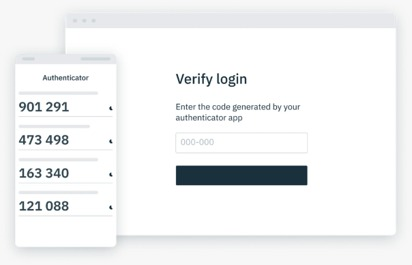
\includegraphics[width=0.7\textwidth]{Imagens/login.jpeg}\\[0.1cm]
\textit{Figura 1: Geração de código temporário com tecnologia TOTP}\par}

\hspace{1cm} Introduz-se a palavra-passe, o sistema valida as credenciais normais e gera um código usando um segredo partilhado e o intervalo de tempo atual. Após o utilizador introduzir o código, o sistema calcula o código esperado e compara os valores, validando deste modo o utilizador dentro da janela esperada e sem repetições.

\hspace{1cm} Existe uma chave secreta conhecida pela aplicação autenticadora e pelo servidor, sendo também usados o tempo atual e um intervalo para calcular o espaço de tempo em que o código é válido. A chave e o valor temporal são passados então a uma função para produzir o código.

\hspace{1cm} O TOTP reforça a segurança da autenticação, mas continua vulnerável a ataques de \textit{phishing}. A sua eficácia depende da proteção do segredo partilhado e da correta sincronização dos relógios.

\subsection{FIDO2 \& WebAuthn}

\hspace{1cm} A tecnologia \textbf{FIDO2}, através do \textbf{WebAuthn}, permite autenticar utilizadores usando criptografia de chave pública, reduzindo a dependência de palavras-passe e reforçando a segurança do processo de autenticação.

\hspace{1cm} O utilizador regista um autenticador, como um sensor biométrico integrado no dispositivo ou uma chave de segurança física. Durante este processo, é criado um par de chaves criptográficas associado ao serviço: uma chave privada, que permanece protegida no autenticador, e uma chave pública, que é armazenada pelo servidor.

{\centering 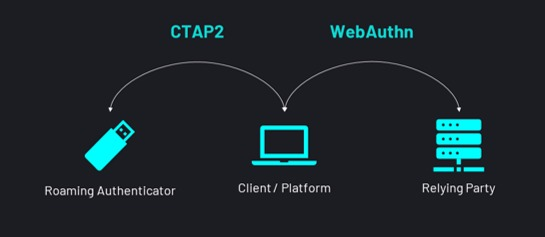
\includegraphics[width=0.7\textwidth]{Imagens/Web.jpeg}\\[0.1cm]
\textit{Figura 2: Arquitetura do FIDO2}\par }

\hspace{1cm} O FIDO2 resulta da combinação de duas especificações complementares: o \textbf{WebAuthn}, que define a interface entre o serviço web e o \textit{browser}, e o \textbf{CTAP2}, que define a comunicação entre o dispositivo do utilizador e o autenticador. Quando o autenticador é externo, como uma chave de segurança física, é o CTAP2 que permite ao \textit{browser} ou ao sistema operativo comunicar com ele por USB, NFC ou \textit{Bluetooth}, pedindo a criação de credenciais e a assinatura de desafios. No caso dos autenticadores integrados no dispositivo, esta comunicação é tratada pelo próprio sistema operativo. Assim, o serviço web interage apenas com o WebAuthn, e os detalhes da comunicação com o autenticador ficam a cargo do CTAP2, o que permite utilizar autenticadores de diferentes fabricantes de forma interoperável.

\hspace{1cm} O servidor envia um desafio criptográfico único, que o autenticador assina com a chave privada após a autorização do utilizador. O servidor verifica a assinatura através da chave pública previamente registada, confirmando a autenticidade da resposta. Adicionalmente, o WebAuthn associa as credenciais ao domínio legítimo do serviço, dificultando a utilização das mesmas em páginas fraudulentas e reforçando a proteção contra ataques de \textit{phishing}.

\hspace{1cm} A sua eficácia depende da proteção das credenciais, da segurança do dispositivo e da implementação correta do protocolo.

\subsection{Autenticação através de aplicações móveis e notificações push}
 
\hspace{1cm} As aplicações de autenticação móveis, como o Microsoft Authenticator ou o Google Authenticator, transformam o telemóvel do utilizador num fator de autenticação da categoria ``algo que se possui'', de forma a verificar que o utilizador é, de facto, o proprietário da conta que tenta autenticar-se. Depois de associada à conta, a aplicação passa a servir de segundo fator no início de sessão, através de dois mecanismos principais: a geração de códigos temporários e o envio de notificações \textit{push} para aprovação do acesso. Ao contrário do SMS, estes mecanismos não dependem da rede móvel para a entrega da mensagem, o que reduz a exposição a certos ataques sobre o canal de comunicação. O estudo de Meyer et al. (2023) mostra que aplicações dedicadas, como o Microsoft Authenticator, oferecem mais proteção do que o SMS.
 
\hspace{1cm} Nas notificações \textit{push}, o serviço envia um pedido de aprovação para o dispositivo registado e o utilizador apenas decide se aceita ou não o início de sessão. Este método é rápido e não exige a introdução de códigos, o que melhora a experiência de utilização. No entanto, a simplicidade da aprovação é também a sua principal fragilidade. Num ataque de \textit{MFA fatigue}, também conhecido como \textit{push bombing}, o atacante que já possui a palavra-passe da vítima tenta repetidamente iniciar sessão, gerando uma sucessão de notificações no dispositivo do utilizador até que este aprove uma delas por engano ou por cansaço.
 
\hspace{1cm} Um dos casos mais conhecidos em que o mecanismo de defesa eram as notificações \textit{push} é o ataque à Uber, em setembro de 2022. Segundo o TechCrunch (2022), o atacante terá obtido acesso aos sistemas internos através da engenharia social de um prestador de serviços. De acordo com os relatos do incidente, o atacante bombardeou o prestador de serviços com notificações \textit{push} e contactou-o depois através do WhatsApp, fazendo-se passar pelo apoio informático da Uber e pedindo-lhe que aprovasse uma das notificações. O prestador aprovou o pedido, o que deu ao atacante acesso à rede interna. Este caso mostra que a falha não esteve na tecnologia em si, mas na forma como a aprovação simples permite que o fator humano seja explorado.
 
\hspace{1cm} Para reduzir este risco, a CISA (2022b) recomenda a utilização de \textit{number matching}, em que o utilizador tem de introduzir na aplicação um número apresentado no ecrã de início de sessão. Desta forma, a aprovação deixa de ser um gesto automático e só quem está a iniciar a sessão consegue concluí-la. Contudo, a CISA (2022a) considera este método apenas uma solução intermédia e recomenda que as organizações migrem para MFA baseada em FIDO/WebAuthn.
 
\hspace{1cm} Em síntese, as aplicações de autenticação oferecem um equilíbrio favorável entre segurança, custo e facilidade de utilização, sendo claramente preferíveis ao SMS e à autenticação por um único fator. Os códigos temporários são simples e funcionam sem ligação à Internet, enquanto as notificações \textit{push} proporcionam maior comodidade, desde que estejam acompanhadas de mecanismos como o \textit{number matching}. Ambos os métodos dependem, contudo, da segurança do dispositivo móvel e exigem processos de recuperação de conta caso o utilizador perca o telemóvel. Em contextos de risco elevado, como contas de administração ou sistemas com informação sensível, justifica-se o recurso a métodos resistentes a \textit{phishing}.

\subsection{Códigos de utilização única por SMS}

\hspace{1cm} A autenticação através de códigos enviados por SMS é um método frequentemente utilizado na autenticação multifator, no qual o utilizador recebe, por mensagem de texto, um código temporário enviado pelo serviço a que pretende aceder. Após introduzir as suas credenciais habituais, como o nome de utilizador e a palavra-passe, o utilizador insere o código recebido no telemóvel para concluir o processo de autenticação. Com isto, acrescenta-se uma etapa de verificação associada ao acesso a um dispositivo que, em princípio, se encontra na posse do utilizador, dificultando o acesso não autorizado quando apenas a palavra-passe é comprometida.

\hspace{1cm} Uma das principais vantagens deste método é a facilidade com que esta se usa e se implementa em serviços. Como não exige necessariamente a instalação de aplicações específicas ou a aquisição de dispositivos adicionais, pode ser uma solução acessível para um elevado número de utilizadores. Contudo, a utilização de SMS apresenta limitações de segurança que devem ser consideradas na escolha de um mecanismo de autenticação. Entre os riscos encontram-se a mudança de um cartão SIM para um dispositivo controlado por terceiros, a exploração de vulnerabilidades nas redes de telecomunicações e a possibilidade de um utilizador ser induzido a revelar o código recebido através de técnicas de engenharia social.

\hspace{1cm} De acordo com o NIST, na publicação \textit{Digital Identity Guidelines: Authentication and Authenticator Management} (SP 800-63B-4), a utilização da rede telefónica pública para a transmissão de códigos de autenticação é considerada um mecanismo de utilização restrita. O documento recomenda que sejam considerados indicadores de risco, como a substituição do cartão SIM, a alteração do número de telemóvel ou a portabilidade recente do número, antes de recorrer a este canal. O NIST salienta ainda a importância de obter métodos alternativos de autenticação, para quando o acesso à rede teleónica não está disponível. Além disso, os códigos introduzidos manualmente, como os recebidos por SMS, não são resistentes a ataques de phishing podendo ser obtidos por um atacante.

\hspace{1cm} Assim, embora a autenticação por SMS possa representar uma melhoria face à utilização exclusiva de uma palavra-passe, não deve ser considerada a melhor opção para proteger contas ou recursos de elevada sensibilidade.

\subsection{Smart Cards}

\hspace{1cm} Os Smart Cards são dispositivos físicos que armazenam credenciais eletrónicas utilizadas para verificar a identidade de um utilizador e controlar o acesso a sistemas ou instalações. No documento \textit{Personal Identity Verification (PIV) of Federal Employees and Contractors} (FIPS 201-3), o NIST descreve que a utilização de cartões PIV serve para autenticação de funcionários e prestadores de serviços do governo federal dos Estados Unidos, tanto no acesso físico como no acesso a recursos informáticos.

\hspace{1cm} De acordo com a secção 6.2.3.1 do FIPS 201-3, no mecanismo de autenticação PKI-AUTH, o sistema lê e valida o certificado de autenticação do cartão, solicita ao utilizador um PIN para o ativar e envia-lhe um desafio criptográfico. O cartão assina esse desafio com a chave privada armazenada, permitindo ao sistema verificar a resposta através da chave pública associada ao certificado. Se a validação for bem-sucedida, a identidade autenticada pode ser utilizada para determinar se o acesso deve ser autorizado.

\hspace{1cm} Os cartões inteligentes podem suportar MFA quando são combinados fatores de autenticação distintos. Por exemplo, a apresentação do cartão corresponde a algo que o utilizador possui, enquanto a introdução de um PIN corresponde a algo que sabe. A exigência destes dois elementos dificulta a utilização indevida de um cartão perdido ou roubado, uma vez que a posse do cartão, por si só, não é suficiente para concluir o mecanismo de validação do utilizador. No entanto, nem todos os cartões inteligentes exigem dois fatores, pelo que a sua utilização nem sempre constitui automaticamente autenticação multifator.

\hspace{1cm} Uma das principais vantagens dos cartões inteligentes é a possibilidade de recorrer a mecanismos criptográficos para verificar a autenticidade das credenciais, reduzindo a dependência de palavras-passe como único meio de autenticação. No mecanismo PKI-AUTH, o NIST destaca a elevada resistência à falsificação de credenciais, a resistência à utilização do cartão por pessoas que não sejam os seus titulares e a possibilidade de verificar se o certificado foi revogado. Além disso, os cartões PIV podem suportar diferentes mecanismos de autenticação permitindo adaptar o nível de garantia às necessidades de segurança do contexto.

\hspace{1cm} Porém, a implementação deste tipo de solução pode exigir leitores compatíveis, sistemas de gestão de certificados e mecanismos para verificar o seu estado de validade ou revogação. Estes requisitos podem aumentar os custos de implementação e manutenção, especialmente em organizações com muitos utilizadores. Existe também o risco de perda ou roubo do cartão, pelo que é importante proteger a sua utilização através de mecanismos de ativação, como um PIN, e de procedimentos para bloquear ou revogar credenciais comprometidas. A escolha deste método deve, por isso, considerar o nível de segurança pretendido, a infraestrutura e os recursos disponível para a sua gestão.

\hspace{1cm} Resumindo, os cartões inteligentes constituem uma boa solução para cenários que exigem uma autenticação robusta, sobretudo quando utilizam credenciais criptográficas e são combinados com um PIN ou outro fator independente. A sua adoção depende, contudo, do contexto de utilização e dos requisitos de segurança, devendo a organização avaliar se os benefícios justificam os custos e a complexidade de implementação.

\subsection{Autenticação biométrica}

\hspace{1cm} A autenticação biométrica utiliza características físicas ou comportamentais de um indivíduo para verificar a sua identidade. De acordo com o \textit{National Institute of Standards and Technology} (NIST), na publicação \textit{Digital Identity Guidelines: Authentication and Authenticator Management} (SP 800-63B-4), estas características podem incluir impressões digitais, características faciais, padrões da íris, padrões de voz ou características comportamentais. Entre os exemplos mais comuns encontram-se o desbloqueio de um dispositivo através da impressão digital ou do reconhecimento facial.

\hspace{1cm} O processo de autenticação começa com a recolha de uma amostra biométrica através de um sensor, como uma câmara ou um leitor de impressões digitais. Essa amostra é comparada com uma referência biométrica previamente registada, permitindo determinar se existe correspondência suficiente para aceitar a autenticação sendo esta comparação, segundo o NIST, probabilística, o que por esse motivo, os sistemas utilizam limiares de aceitação que procuram equilibrar a segurança e a facilidade de utilização.

\hspace{1cm} De acordo com a secção \textit{Use of Biometrics} do SP 800-63B-4, o NIST estabelece que a biometria deve ser utilizada como parte de um processo de autenticação multifator, em conjunto com um autenticador físico, correspondente a algo que o utilizador possui, por exemplo, a posse do dispositivo combinada com a característica biométrica por forma a desbloquear o acesso a um local/serviço.

\hspace{1cm} A principal vantagem da autenticação biométrica é que esta proporciona uma experiência de utilização rápida e conveniente, reduzindo a necessidade de memorizar e introduzir palavras-passe ou códigos, pode também facilitar a utilização frequente de mecanismos de MFA, uma vez que o utilizador pode confirmar a sua identidade através de uma característica que lhe é própria.

\hspace{1cm} Apesar das suas vantagens, a autenticação biométrica apresenta limitações relacionadas com a precisão, a privacidade e a resistência a ataques. Situações como esta podem ocorrer, por exemplo, devido a alterações na iluminação durante o reconhecimento facial, à presença de humidade ou sujidade nos dedos ou a lesões que afetem a leitura das impressões digitais. Outra limitação relevante diz respeito à proteção dos dados biométricos. Ao contrário de uma palavra-passe, uma característica física não pode ser facilmente alterada caso seja comprometida. Por esse motivo, o NIST determina que os dados biométricos sejam tratados e protegidos como informação pessoal sensível.

\hspace{1cm} Por fim, a autenticação biométrica pode contribuir para uma experiência de autenticação mais simples e para o reforço da segurança, desde que seja integrada num mecanismo de MFA adequado. A sua implementação deve ter em conta a precisão do sistema, a proteção dos dados pessoais, a resistência a ataques e a disponibilidade de métodos alternativos. Desta forma, a escolha da biometria deve considerar tanto o nível de segurança pretendido como as necessidades e limitações dos utilizadores.

\subsection{Comparação entre as tecnologias analisadas}

\hspace{1cm} A comparação entre as várias tecnologias apresentadas anteriormente apresentam-se na Tabela \ref{tab:comparacao-tecnologias-mfa} onde se demonstra cada tecnologia, o seu funcionamento, vantagens e as suas limitações.

\begin{table}[htbp]
\centering
\scriptsize
\setlength{\tabcolsep}{4pt}
\renewcommand{\arraystretch}{1.1}

\begin{tabularx}{\textwidth}{|>{\raggedright\arraybackslash}p{2.2cm}|X|X|X|}
\hline
\textbf{Tecnologia} & \textbf{Funcionamento} & \textbf{Vantagens} & \textbf{Limitações} \\
\hline
TOTP &
Gera códigos temporários através de uma aplicação e de uma chave partilhada. &
Funciona sem ligação à Internet no momento da geração do código. &
Os códigos podem ser roubados através de phishing. \\
\hline
FIDO2 / WebAuthn &
Utiliza chaves criptográficas para autenticar o utilizador. &
Elevada resistência a phishing e não exige a introdução de códigos. &
A compatibilidade e a configuração podem variar consoante os dispositivos e serviços. \\
\hline
Aplicações móveis e notificações push &
Envia uma notificação para um dispositivo registado, solicitando a aprovação do acesso. &
Utilização simples e rápida. &
Pode ser vulnerável a aprovações indevidas ou a ataques de fadiga de MFA. \\
\hline
SMS &
Envia um código temporário por mensagem de texto. &
Fácil de utilizar e amplamente acessível. &
Vulnerável a troca de SIM, engenharia social e phishing. \\
\hline
Smart Cards &
Utiliza um cartão físico com credenciais, podendo exigir um PIN. &
Permite autenticação criptográfica robusta e controlo de acesso. &
Pode exigir leitores, infraestrutura específica e gestão de certificados. \\
\hline
Biometria &
Compara características físicas, como a impressão digital ou o rosto. &
Rápida e conveniente para o utilizador. &
Pode apresentar erros de reconhecimento e riscos de privacidade. \\
\hline
\end{tabularx}

\caption{Comparação entre tecnologias de autenticação multifator.}
\label{tab:comparacao-tecnologias-mfa}
\end{table}